\documentclass[11pt]{article}

\usepackage[utf8]{inputenc}
\usepackage{amsmath}
\usepackage{graphicx}
\usepackage{booktabs}
\usepackage{float}
\usepackage{hyperref}
\usepackage{geometry}
\usepackage{caption}
\geometry{margin=1in}

\title{Dry Waste Image Classification Dataset \\ \large Dataset Documentation and Baseline Evaluation}
\author{Kamal Jannati}
\date{\today}

\begin{document}
\maketitle

\begin{abstract}
This document describes a dataset of single-item dry waste images collected in 2020 using a purpose-built automated waste-sorting device. The dataset contains 2{,}043 images across three material categories: metal, paper, and plastic. To validate that the dataset carries meaningful, learnable signal, a lightweight transfer-learning classifier (MobileNetV2, partially fine-tuned) was trained on the data as a sanity check, achieving 82.3\% overall accuracy on a held-out validation split. This result is presented as evidence that the dataset trains a real classifier reasonably well, \emph{not} as a tuned or state-of-the-art benchmark; no extensive hyperparameter search or architecture comparison was performed. This document is intended to accompany the public release of the dataset and serves as its dataset card / datasheet.
\end{abstract}

\tableofcontents

% ============================================================
\section{Motivation and Background}
% ============================================================

The dataset was originally collected as part of a 2020 project to build an automated dry-waste sorting machine using machine learning and image processing. A physical device was constructed to photograph individual waste items in a fixed top-down orientation against a consistent background, enabling controlled, low-variance image capture across four candidate categories: glass, metal, paper, and plastic.

The original hardware project did not reach completion and the physical device was subsequently decommissioned. The image dataset, however, remains intact and is released here to allow reuse by others working on waste classification, recycling automation, or as a lightweight benchmark dataset for transfer-learning experiments.

\subsection{Note on the Glass Category}
The original device also captured a small number of glass images. However, only 22 glass images were collected in total (18 train / 4 validation after splitting), which is insufficient for meaningful training or evaluation. The glass category has therefore been \textbf{excluded} from this release. Users requiring a glass class should be aware it is not represented in this dataset.

% ============================================================
\section{Data Collection}
% ============================================================

\subsection{Acquisition Setup}
Images were captured using a fixed-position camera mounted above a transparent viewing panel inside the sorting device. Each image contains a single waste item, photographed from directly above under consistent (though not perfectly controlled) ambient lighting. The background is a light-colored panel visible in all images, along with minor consistent artifacts (mounting screws, surface marks, occasional glare) inherent to the physical device.

% TODO: fill in any additional details you recall, e.g. camera model/resolution,
% approximate distance from lens to item, whether lighting was artificial/natural, etc.

\subsection{Class Definitions}
Each image is labeled with exactly one of the following three classes:
\begin{itemize}
    \item \textbf{Metal} --- e.g. beverage cans, metal foil packaging, bottle caps.
    \item \textbf{Paper} --- e.g. cardboard, paper packaging, folded paper items.
    \item \textbf{Plastic} --- e.g. bottles, plastic packaging, plastic lids/containers.
\end{itemize}

% ============================================================
\section{Dataset Statistics}
% ============================================================

\subsection{Class Distribution}

The dataset contains 2{,}043 images in total, split 80/20 into training and validation sets (1{,}636 train / 407 validation). Table~\ref{tab:class-dist} and Figure~\ref{fig:class-dist} show the per-class breakdown.

\begin{table}[H]
\centering
\caption{Per-class image counts.}
\label{tab:class-dist}
\begin{tabular}{lccc}
\toprule
Class & Train & Validation & Total \\
\midrule
Metal   & 604 & 151 & 755 \\
Paper   & 464 & 115 & 579 \\
Plastic & 568 & 141 & 709 \\
\midrule
\textbf{Total} & \textbf{1{,}636} & \textbf{407} & \textbf{2{,}043} \\
\bottomrule
\end{tabular}
\end{table}

\begin{figure}[H]
\centering
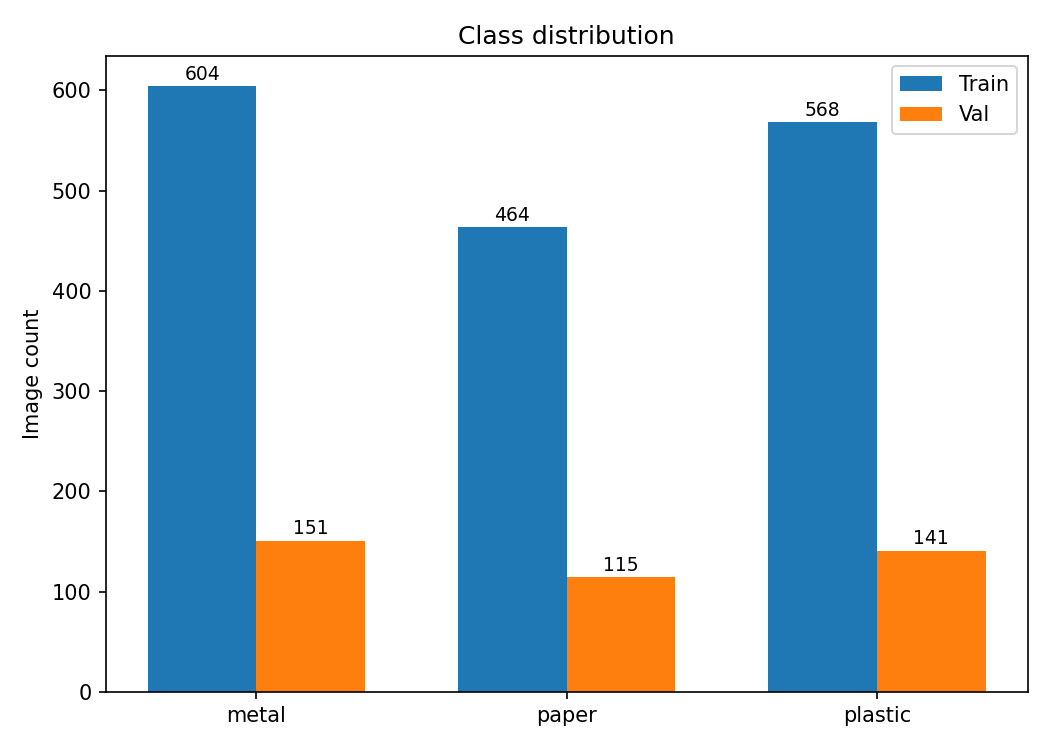
\includegraphics[width=0.75\textwidth]{figures/class_distribution.png}
\caption{Train/validation image counts per class.}
\label{fig:class-dist}
\end{figure}

The dataset is moderately imbalanced, with paper underrepresented (579 images, 28.3\% of the dataset) relative to metal (755 images, 37.0\%) and plastic (709 images, 34.7\%). This imbalance is discussed further in Section~\ref{sec:results} in the context of baseline model performance.

\subsection{Sample Images}

Figure~\ref{fig:samples} shows representative example images from each class, illustrating typical item appearance, scale, and the consistent capture background.

\begin{figure}[H]
\centering
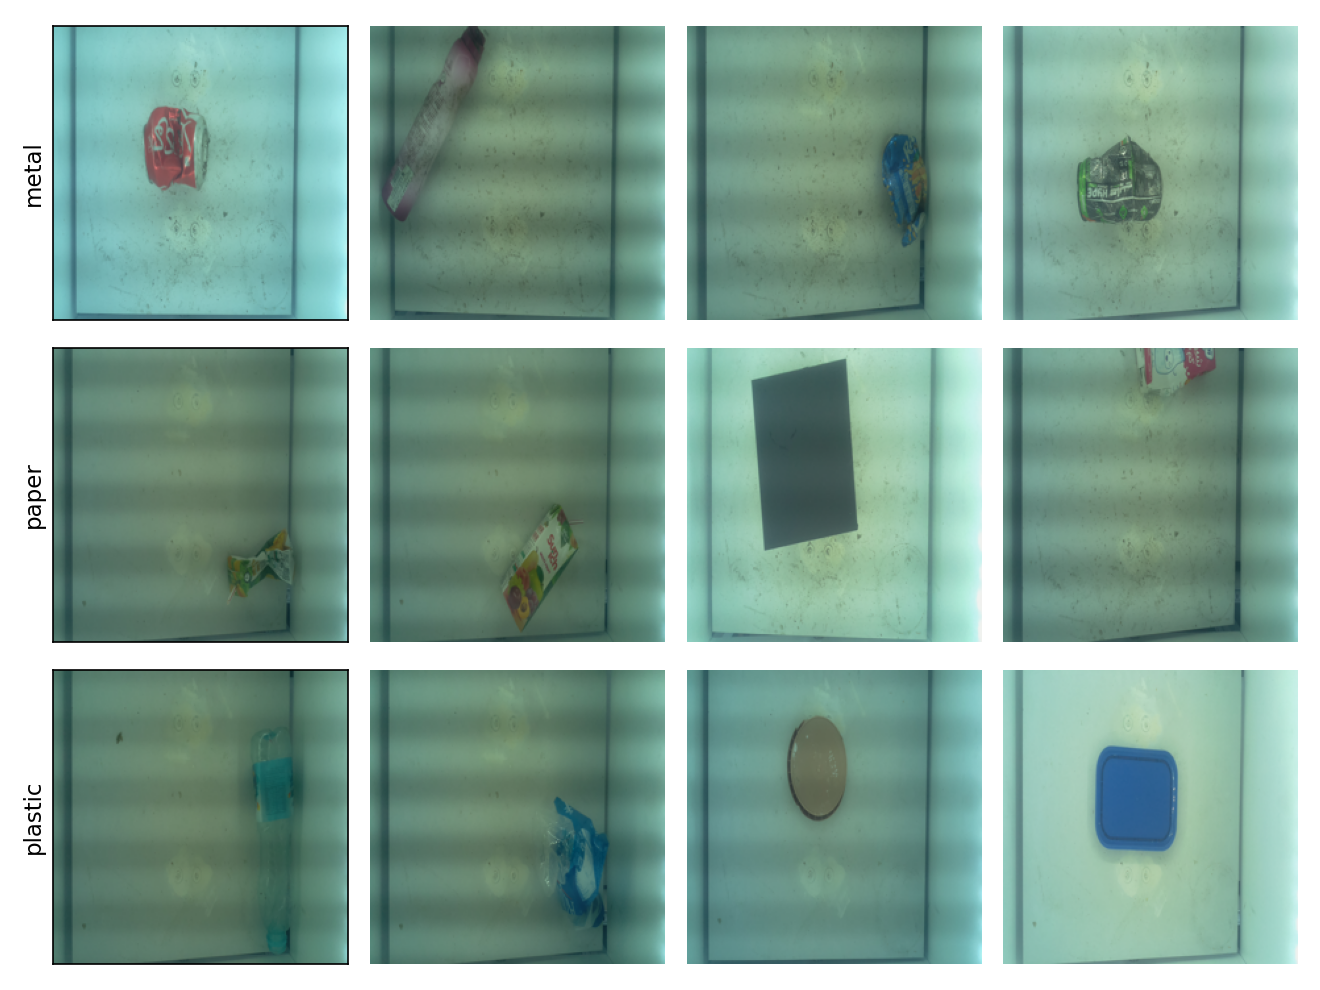
\includegraphics[width=0.8\textwidth]{figures/sample_grid.png}
\caption{Example images from each of the three classes.}
\label{fig:samples}
\end{figure}

% ============================================================
\section{Baseline Validation Experiment}
% ============================================================

The purpose of this experiment is \emph{not} to produce a state-of-the-art waste classifier, but to sanity-check the dataset: to confirm that the images are consistently labeled, visually distinguishable across classes, and sufficient in quantity to train a real classifier above chance level. A single, modestly-tuned transfer-learning baseline was trained and evaluated for this purpose.

\subsection{Architecture and Training Setup}
\begin{itemize}
    \item \textbf{Base architecture:} MobileNetV2, pretrained on ImageNet.
    \item \textbf{Fine-tuning strategy:} The final two feature blocks of the backbone and the classifier head were fine-tuned; earlier layers remained frozen. A differential learning rate was used (backbone: $\text{LR} \times 0.1$, classifier head: full LR).
    \item \textbf{Input resolution:} $224 \times 224$.
    \item \textbf{Augmentation:} Random resized crop, horizontal flip, random rotation ($\pm 15^\circ$), and color jitter (brightness/contrast/saturation).
    \item \textbf{Optimizer:} Adam, with a \texttt{ReduceLROnPlateau} learning-rate scheduler.
    \item \textbf{Early stopping:} Training halted after 5 epochs without validation improvement.
\end{itemize}

% TODO: if you re-run with different hyperparameters (e.g. more unfrozen blocks,
% class weighting), update this subsection accordingly.

\subsection{Results}
\label{sec:results}

The best model, selected by validation accuracy, achieved \textbf{82.3\% overall accuracy} on the held-out validation set. This confirms the dataset trains a real classifier well above the 33\% chance level for a 3-class problem, and supports its use as a viable dataset for further work. The result should be read as confirmation that the data carries strong, learnable signal --- not as a fully optimized or maximal-accuracy benchmark, since no hyperparameter search, architecture comparison, or extensive fine-tuning was performed. Table~\ref{tab:report} and Figure~\ref{fig:curves} give per-class and training-progression detail.

\begin{table}[H]
\centering
\caption{Per-class classification metrics on the validation set.}
\label{tab:report}
\begin{tabular}{lcccc}
\toprule
Class & Precision & Recall & F1-score & Support \\
\midrule
Metal   & 0.771 & 0.914 & 0.836 & 151 \\
Paper   & 0.928 & 0.783 & 0.849 & 115 \\
Plastic & 0.817 & 0.759 & 0.787 & 141 \\
\midrule
\textbf{Accuracy}     & \multicolumn{3}{c}{0.823} & 407 \\
\textbf{Macro avg}    & 0.839 & 0.818 & 0.824 & 407 \\
\textbf{Weighted avg} & 0.831 & 0.823 & 0.823 & 407 \\
\bottomrule
\end{tabular}
\end{table}

\begin{figure}[H]
\centering
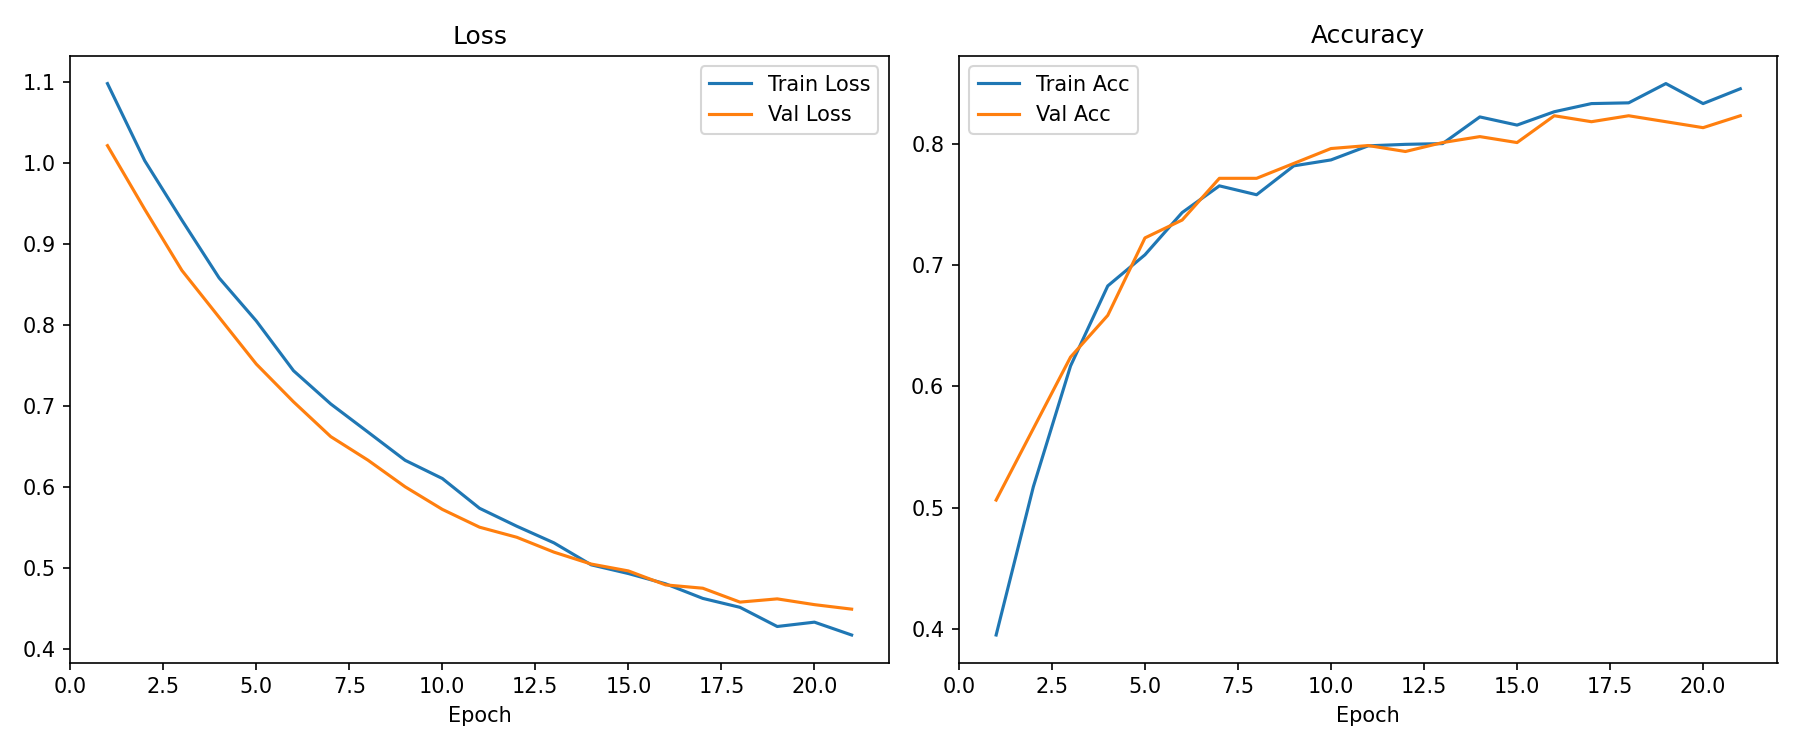
\includegraphics[width=\textwidth]{figures/training_curves.png}
\caption{Training and validation loss (left) and accuracy (right) over training epochs.}
\label{fig:curves}
\end{figure}

\begin{figure}[H]
\centering
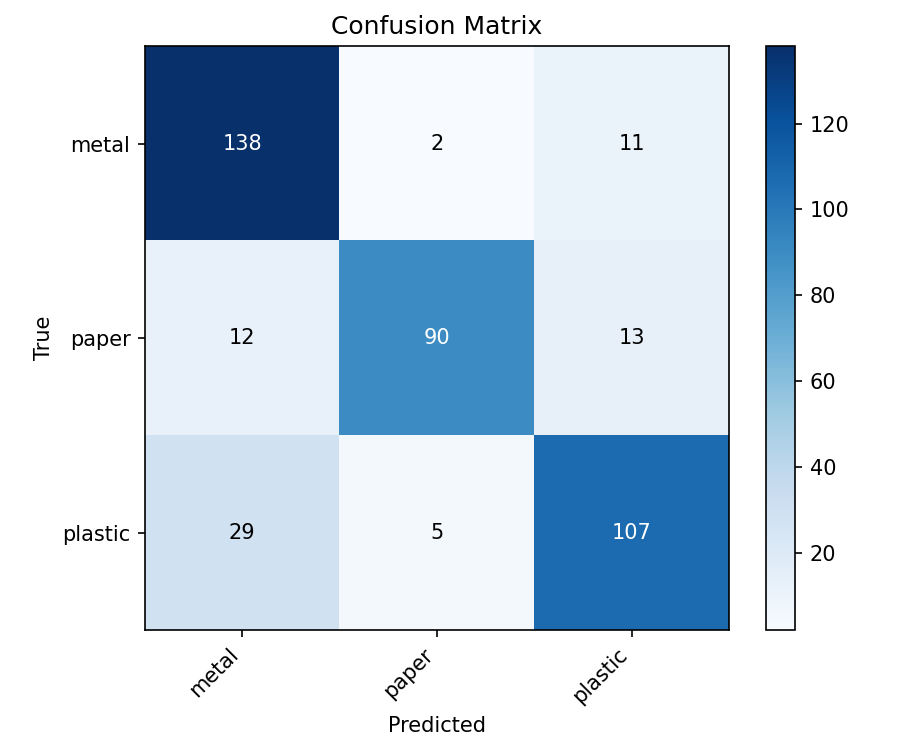
\includegraphics[width=0.65\textwidth]{figures/confusion_matrix.png}
\caption{Validation set confusion matrix.}
\label{fig:confmat}
\end{figure}

\subsection{Discussion}

The training and validation loss/accuracy curves (Figure~\ref{fig:curves}) track closely throughout training, with no evidence of overfitting; validation accuracy plateaus around epoch 20, consistent with the early-stopping trigger.

The confusion matrix (Figure~\ref{fig:confmat}) highlights the main source of error: 29 plastic images were misclassified as metal, the single largest off-diagonal error in the matrix. Metal achieves the highest recall (0.914) but the lowest precision (0.771) of the three classes, indicating the model over-predicts metal, partly at the expense of plastic. Paper shows the opposite pattern (highest precision, 0.928; lower recall, 0.783), suggesting the model is conservative about predicting paper, consistent with paper being the least-represented class in the training set (Table~\ref{tab:class-dist}).

% TODO: add any qualitative observations of your own, e.g. specific items that
% seem to consistently confuse the model (e.g. shiny plastic packaging vs metal foil).

% ============================================================
\section{Known Limitations}
% ============================================================

\begin{itemize}
    \item \textbf{Single-device capture:} All images originate from one physical device with a fixed camera position and background. Models trained on this dataset alone may not generalize well to other capture setups, lighting conditions, or backgrounds.
    \item \textbf{Glass excluded:} As noted in Section~\ref{sec:glass}, glass was collected but is not included due to insufficient sample count (22 images).
    \item \textbf{Class imbalance:} Paper is moderately underrepresented relative to metal and plastic (Table~\ref{tab:class-dist}).
    \item \textbf{Single item per image:} All images depict a single waste item; the dataset does not cover multi-item scenes, occlusion, or cluttered backgrounds.
    \item \textbf{Dataset size:} At just over 2{,}000 images, the dataset is small relative to large-scale vision benchmarks, though comparable to or larger than some existing public waste-classification datasets (e.g. TrashNet, $\sim$2{,}500 images across 6 classes).
\end{itemize}
\label{sec:glass}

% ============================================================
\section{Licensing and Citation}
% ============================================================

% TODO: finalize license choice and citation details before publishing.

\subsection{License}
This dataset is released under the \textbf{Creative Commons Attribution 4.0 International (CC BY 4.0)} license. Users are free to share and adapt the material for any purpose, including commercially, provided appropriate credit is given.

\subsection{Suggested Citation}
\begin{quote}
\itshape
Jannati, K. (2026). Dry Waste Classification Dataset (Metal, Paper,
Plastic) [Data set]. Zenodo. https://doi.org/10.5281/zenodo.21849964
\end{quote}

\subsection{Accompanying Code}
A baseline training script (PyTorch, MobileNetV2 transfer learning) is released alongside this dataset and is licensed separately under the \textbf{MIT License}.

\begin{itemize}
    \item \textbf{GitHub repository:} \url{https://github.com/Kamaljust/dry-waste-classification-dataset}
    \item \textbf{Dataset DOI (Zenodo):} \url{https://doi.org/10.5281/zenodo.21849964}
\end{itemize}

% ============================================================
\section{Contact}
% ============================================================
Kamal Jannati --- \url{https://github.com/Kamaljust}

\end{document}
